% $Id: template.tex 11 2007-04-03 22:25:53Z jpeltier $

\documentclass{vgtc}                          % final (conference style)
% \documentclass[review]{vgtc}                % review
%\documentclass[widereview]{vgtc}             % wide-spaced review
%\documentclass[preprint]{vgtc}               % preprint
%\documentclass[electronic]{vgtc}             % electronic version

%% Uncomment one of the lines above depending on where your paper is
%% in the conference process. ``review'' and ``widereview'' are for review
%% submission, ``preprint'' is for pre-publication, and the final version
%% doesn't use a specific qualifier. Further, ``electronic'' includes
%% hyperreferences for more convenient online viewing.

%% Please use one of the ``review'' options in combination with the
%% assigned online id (see below) ONLY if your paper uses a double blind
%% review process. Some conferences, like IEEE Vis and InfoVis, have NOT
%% in the past.

%% Figures should be in CMYK or Grey scale format, otherwise, colour 
%% shifting may occur during the printing process.

%% it is recomended to use ``\cref{sec:bla}'' instead of ``Fig.~\ref{sec:bla}''
\graphicspath{{figures/}{pictures/}{images/}{./}} % where to search for the images

\usepackage{times}                     % we use Times as the main font
\renewcommand*\ttdefault{txtt}         % a nicer typewriter font

%% Only used in the template examples. You can remove these lines.
\usepackage{tabu}                      % only used for the table example
\usepackage{booktabs}                  % only used for the table example
\usepackage{lipsum}                    % used to generate placeholder text
\usepackage{mwe}                       % used to generate placeholder figures

%% We encourage the use of mathptmx for consistent usage of times font
%% throughout the proceedings. However, if you encounter conflicts
%% with other math-related packages, you may want to disable it.
\usepackage{mathptmx}                  % use matching math font


%% If you are submitting a paper to a conference for review with a double
%% blind reviewing process, please replace the value ``0'' below with your
%% OnlineID. Otherwise, you may safely leave it at ``0''.
\onlineid{0}

%% declare the category of your paper, only shown in review mode
\vgtccategory{Research}

%% allow for this line if you want the electronic option to work properly
\vgtcinsertpkg

%% In preprint mode you may define your own headline. If not, the default IEEE copyright message will appear in preprint mode.
%\preprinttext{To appear in an IEEE VGTC sponsored conference.}

%% This adds a link to the version of the paper on IEEEXplore
%% Uncomment this line when you produce a preprint version of the article 
%% after the article receives a DOI for the paper from IEEE
%\ieeedoi{xx.xxxx/TVCG.201x.xxxxxxx}


%% Paper title.

\title{Interactive Visualization of Time-Dependent Bipartite Graphs}

%% This is how authors are specified in the conference style

%% Author and Affiliation (single author).
% \author{Yahya Jabary\thanks{e-mail:yahya.jabary@tuwien.ac.at}}
% \affiliation{\scriptsize TU Wien}

%% Author and Affiliation (multiple authors with single affiliations).
\author{Yahya Jabary\thanks{e-mail:yahya.jabary@tuwien.ac.at} %
% \and Manuela Waldner,\thanks{e-mail:manuela.waldner@tuwien.ac.at} %
\and Manuela Waldner\thanks{e-mail:manuela.waldner@tuwien.ac.at}}
\affiliation{\scriptsize Vienna University of Technology }

%% Author and Affiliation (multiple authors with multiple affiliations)
% \author{Roy G. Biv\thanks{e-mail: roy.g.biv@aol.com}\\ %
%         \scriptsize Starbucks Research %
% \and Ed Grimley\thanks{e-mail: ed.grimley@aol.com}\\ %
%      \scriptsize Grimley Widgets, Inc. %
% \and Martha Stewart\thanks{e-mail: martha.stewart@marthastewart.com}\\ %
%      \parbox{1.4in}{\scriptsize \centering Martha Stewart Enterprises \\ Microsoft Research}}

% --------------------------------------------------------------------------------------------------











































% \teaser{
%   \centering
%   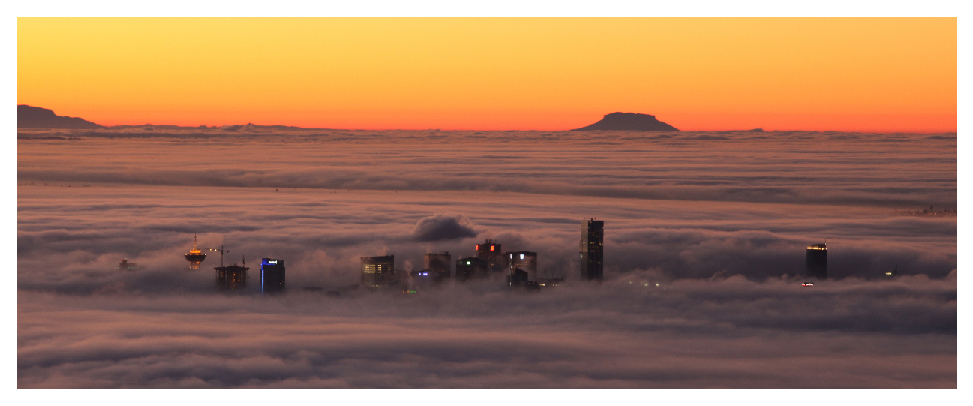
\includegraphics[width=\linewidth]{CypressView}
%   \caption{In the Clouds: Vancouver from Cypress Mountain.}
%   \label{fig:teaser}
% }

% \abstract{
%   write the abstract when you're done with the paper
% }
\keywords{Interactive Visualization, Temporal Graphs, Bipartite Graphs, Transparency Database}
  
\nocopyrightspace
  
\begin{document}
  
\maketitle

% \noindent\hfil\rule{0.2\textwidth}{.4pt}\hfil
% \medskip
% \bigskip











% deadline: 10.7.
% similar to an extended master thesis proposal
% length: 4-5 pages

\section{Introduction} % introduction / general conditions / motivation: which user group / research question do you want to find a solution for. you can define this freely, but you should motivate why the topic is relevant.

Effective visualization of temporal graphs can reveal valuable insights such as patterns, trends, and anomalies that might otherwise remain hidden in raw data. This allows researchers, analysts, and decision-makers to quickly grasp evolving relationships, identify critical points of change, and make data-driven decisions.

In the context of global warming, multi-temporal scale visualizations of carbon emissions data can provide valuable insights for decision-makers, as demonstrated by Ma et al. \cite{ma2023histgnn}. In logistics, these visualizations can help optimize supply chain operations and identify inefficiencies \cite{Yang2019AnimatedMS} \cite{Tamilmani2019ModellingAA}. For social networks, they can illuminate user interactions and information spread. In public policy, temporal graph visualizations can aid in tracking disease spread, monitoring resource allocation and analyzing policy impacts \cite{chung2023temporal}.
These examples demonstrate how temporal graph visualizations compress temporal network data into intuitive representations. And as the volume and complexity of temporal data continue to grow across various domains, the development and application of effective visualization techniques for temporal graphs will likely become increasingly important.

\medskip

As a practical example this paper explores various techniques for interactive visualization of time-dependent and bipartite graphs, using the ``Media Transparency Database Austria'' \cite{dataset}.

\textbf{Time-dependent} graphs or temporal graphs are structures that evolve over time, with nodes and edges changing as time progresses. These graphs are crucial for representing dynamic systems and processes that unfold chronologically. They allow us to observe patterns, trends, and changes in relationships between entities over different time periods \cite{Waldner2020InteractiveEO}.
One specific type of temporal graph that has gained prominence is the bipartite graph. \textbf{Bipartite} graphs or bigraphs consist of two distinct sets of nodes, with connections only existing between nodes from different sets, but not within the same set. If the two subsets have equal cardinality (balanced bigraph) and each node in one subset is connected to every node in the other subset, the graph is called a complete bigraph \cite{diestel2012graph}. These graphs are particularly useful for modeling relationships between two different types of entities, such as public authorities and their advertising expenditures.
Due to their scale and complexity, time-dependent and bipartite graphs can be challenging to visualize effectively. To make sense of the Media Transparency Database Austria, which contains thousands of entries over multiple years, we need to design scalable and \textbf{interactive visualizations} that allow users to explore the data, for example, by filtering, zooming, and selecting specific time periods or entities.

The ``Media Transparency Database Austria'' \cite{dataset} is a public repository that records the advertising expenses of public authorities in Austria. This database serves as a tool for transparency (based on the Austrian § 34 Transparenzdatenbankgesetz 2012 TDBG), allowing citizens and researchers to track how public funds are spent on advertising across various media outlets. It provides a rich dataset that can be represented as both a time-dependent and bipartite graph structure. By visualizing this data \textendash{} although not the focus of this paper \textendash{} we can gain insights into how public authorities allocate advertising budgets, which media outlets receive the most / least funding, how both the political and media landscapes evolve over time and mutually influence each other.

\medskip

This paper aims to combine state-of-the-art techniques and approaches for designing interactive visualizations of time-dependent and bipartite graphs to propose a final design for the ``Media Transparency Database Austria''. We will focus on clear, uncluttered overviews while maximizing information content and propose a design that allows users to interact with the data intuitively. Additionally, we will consider how our proposed visualization could be evaluated and what results we expect to achieve.















\section{Related Work} % which solutions exist, what are their strengths and weaknesses, how suitable are they for the data characteristics of the Media Transparency Database


% Existing visualization methods often struggle with large-scale, temporal bipartite data. Our research aims to address these limitations through:

% 1. Scalable visualization techniques for large datasets
% 2. Hierarchical aggregation and clustering methods
% 3. Intuitive user interface design
% 4. Integration of time series visualization





% The goal is to create accessible, insightful visualizations  will contribute to information visualization research and provide tools for analyzing public spending on advertising in Austria.

% horizon graphs

% [Waldner et al., 2020]: https://users.cg.tuwien.ac.at/~waldner/bicflows/
% https://www.cvast.tuwien.ac.at/topics/media-transparency-dashboard
% https://users.cg.tuwien.ac.at/~waldner/bicflows/bicflows_steinboeck_bdva2018.pdf
% https://www.vrvis.at/publications/pdfs/PB-VRVis-2020-058.pdf
% https://informs-sim.org/wsc03papers/090.pdf
% https://www.sciencedirect.com/science/article/pii/S2590118420300198
% https://lliquid.github.io/homepage/files/draft_vis18_bico.pdf
% https://www.researchgate.net/publication/4053779_Visualization_methods_for_time-dependent_data_-_An_overview
% https://link.springer.com/chapter/10.1007/978-3-642-02577-8_89
% https://ieeexplore.ieee.org/document/1261490
% https://www.semanticscholar.org/paper/Interactive-exploration-of-large-time-dependent-Waldner-Steinb%C3%B6ck/a540758ed137bdfaf20aa5b41c64c66c4c61cb38
% https://www.semanticscholar.org/paper/de72a42b914735fc54702c903bd010516524bafc
% https://www.semanticscholar.org/paper/d1c0933bb3f45274e968d0fc095f7a4ac36c17ee
% https://pubmed.ncbi.nlm.nih.gov/30130217/
% https://www.semanticscholar.org/paper/9c455b697f3dcf1b5876e80961558d2a37e27c1c
% https://www.semanticscholar.org/paper/8cdb4c4a3a9cfd04c04b3844955ddac9323b1bfd
% https://www.semanticscholar.org/paper/de72a42b914735fc54702c903bd010516524bafc
% https://arxiv.org/abs/2302.06286
% https://www.semanticscholar.org/paper/58c63dd15a1e90a0ad71fae47084d32503bf24a4
% https://www.semanticscholar.org/paper/5a05d02e69359333cdf408cd73ceb498157a0ebe

















\section{Visual Encoding and Interaction Design} % which visual encoding and interaction design would you suggest for the Media Transparency Database (a description and possibly a sketch are sufficient); please justify your choice; you can also choose an existing concept from the Related Work and adapt it, with appropriate justification.
















\section{Implementation} % how would you technically implement the visualization solution and what challenges would you expect – Design Justification / Hypothesis Building (part of research process)
















\section{Evaluation} % how would you evaluate that your proposed solution is "good" (plus: how do you define "good"?). What are the expected results?
















































% --------------------------------------------------------------------------------------------------


%% \section{Introduction} %for journal use above \firstsection{..} instead
% This template is for papers of VGTC-sponsored conferences which are \emph{\textbf{not}} published in a special issue of TVCG.

% \section{Using This Template}

% \begin{itemize}
% \item If you receive compilation errors along the lines of ``\texttt{Package ifpdf Error: Name clash, \textbackslash ifpdf is already defined}'' then please add a new line ``\texttt{\textbackslash let\textbackslash ifpdf\textbackslash relax}'' right after the ``\texttt{\textbackslash documentclass[journal]\{vgtc\}}'' call. Note that your error is due to packages you use that define ``\texttt{\textbackslash ifpdf}'' which is obsolete (the result is that \texttt{\textbackslash ifpdf} is defined twice); these packages should be changed to use ifpdf package instead.
% \item The style uses the hyperref package, thus turns references into internal links. We thus recommend to make use of the ``\texttt{\textbackslash cref\{reference\}}'' call (instead of ``\texttt{Figure\~{}\textbackslash ref\{reference\}}'' or similar) since ``\texttt{\textbackslash cref\{reference\}}'' turns the entire reference into an internal link, not just the number. Examples: \cref{fig:vis_papers} and \cref{tab:vis_papers}.
% \item The style automatically looks for image files with the correct extension (eps for regular \LaTeX; pdf, png, and jpg for pdf\LaTeX), in a set of given subfolders (figures/, pictures/, images/). It is thus sufficient to use ``\texttt{\textbackslash includegraphics\{CypressView\}}'' (instead of ``\texttt{\textbackslash includegraphics\{pictures/CypressView.jpg\}}'').
% \item For adding hyperlinks and DOIs to the list of references, you can use ``\texttt{\textbackslash bibliographystyle\{abbrv-doi-hyperref-narrow\}}'' (instead of ``\texttt{\textbackslash bibliographystyle\{abbrv\}}''). It uses the doi and url fields in a bib\TeX\ entry and turns the entire reference into a link, giving priority to the doi. The doi can be entered with or without the ``\texttt{http://dx.doi.org/}'' url part. See the examples in the bib\TeX\ file and the bibliography at the end of this template.\\[1em]
% \textbf{Note 1:} occasionally (for some \LaTeX\ distributions) this hyper-linked bib\TeX\ style may lead to \textbf{compilation errors} (``\texttt{pdfendlink ended up in different nesting level ...}'') if a reference entry is broken across two pages (due to a bug in hyperref). In this case make sure you have the latest version of the hyperref package (i.\,e., update your \LaTeX\ installation/packages) or, alternatively, revert back to ``\texttt{\textbackslash bibliographystyle\{abbrv-doi-narrow\}}'' (at the expense of removing hyperlinks from the bibliography) and try ``\texttt{\textbackslash bibliographystyle\{abbrv-doi-hyperref-narrow\}}'' again after some more editing.\\[1em]
% \textbf{Note 2:} the ``\texttt{-narrow}'' versions of the bibliography style use the font ``PTSansNarrow-TLF'' for typesetting the DOIs in a compact way. This font needs to be available on your \LaTeX\ system. It is part of the \href{https://www.ctan.org/pkg/paratype}{``paratype'' package}, and many distributions (such as MikTeX) have it automatically installed. If you do not have this package yet and want to use a ``\texttt{-narrow}'' bibliography style then use your \LaTeX\ system's package installer to add it. If this is not possible you can also revert to the respective bibliography styles without the ``\texttt{-narrow}'' in the file name.\\[1em]
% DVI-based processes to compile the template apparently cannot handle the different font so, by default, the template file uses the \texttt{abbrv-doi} bibliography style but the compiled PDF shows you the effect of the \texttt{abbrv-doi-hyperref-narrow} style.
% \end{itemize}

% \section{Bibliography Instructions}

% \begin{itemize}
% \item Sort all bibliographic entries alphabetically but the last name of the first author. This \LaTeX/bib\TeX\ template takes care of this sorting automatically.
% \item Merge multiple references into one; e.\,g., use \cite{Kitware:2003,Max:1995:OMF} (not \cite{Kitware:2003}\cite{Max:1995:OMF}). Within each set of multiple references, the references should be sorted in ascending order. This \LaTeX/bib\TeX\ template takes care of both the merging and the sorting automatically.
% \item Verify all data obtained from digital libraries, even ACM's DL and IEEE Xplore  etc.\ are sometimes wrong or incomplete.
% \item Do not trust bibliographic data from other services such as Mendeley.com, Google Scholar, or similar; these are even more likely to be incorrect or incomplete.
% \item Articles in journal---items to include:
%   \begin{itemize}
%   \item author names
% 	\item title
% 	\item journal name
% 	\item year
% 	\item volume
% 	\item number
% 	\item month of publication as variable name (i.\,e., \{jan\} for January, etc.; month ranges using \{jan \#\{/\}\# feb\} or \{jan \#\{-{}-\}\# feb\})
%   \end{itemize}
% \item use journal names in proper style: correct: ``IEEE Transactions on Visualization and Computer Graphics'', incorrect: ``Visualization and Computer Graphics, IEEE Transactions on''
% \item Papers in proceedings---items to include:
%   \begin{itemize}
%   \item author names
% 	\item title
% 	\item abbreviated proceedings name: e.\,g., ``Proc.\textbackslash{} CONF\_ACRONYNM'' without the year; example: ``Proc.\textbackslash{} CHI'', ``Proc.\textbackslash{} 3DUI'', ``Proc.\textbackslash{} Eurographics'', ``Proc.\textbackslash{} EuroVis''
% 	\item year
% 	\item publisher
% 	\item town with country of publisher (the town can be abbreviated for well-known towns such as New York or Berlin)
%   \end{itemize}
% \item article/paper title convention: refrain from using curly brackets, except for acronyms/proper names/words following dashes/question marks etc.; example:
% \begin{itemize}
% 	\item paper ``Marching Cubes: A High Resolution 3D Surface Construction Algorithm''
% 	\item should be entered as ``\{M\}arching \{C\}ubes: A High Resolution \{3D\} Surface Construction Algorithm'' or  ``\{M\}arching \{C\}ubes: A high resolution \{3D\} surface construction algorithm''
% 	\item will be typeset as ``Marching Cubes: A high resolution 3D surface construction algorithm''
% \end{itemize}
% \item for all entries
% \begin{itemize}
% 	\item DOI can be entered in the DOI field as plain DOI number or as DOI url; alternative: a url in the URL field
% 	\item provide full page ranges AA-{}-BB
% \end{itemize}
% \item when citing references, do not use the reference as a sentence object; e.\,g., wrong: ``In \cite{Lorensen:1987:MCA} the authors describe \dots'', correct: ``Lorensen and Cline \cite{Lorensen:1987:MCA} describe \dots''
% \end{itemize}

% \section{Supplemental Material Instructions}
% \label{sec:supplement_inst}

% In support of transparent research practices and long-term open science goals, you are encouraged to make your supplemental materials available on a publicly-accessible repository.
% Please describe the available supplemental materials in the \hyperref[sec:supplemental_materials]{Supplemental Materials} section.
% These details could include (1) what materials are available, (2) where they are hosted, and (3) any necessary omissions.

% \section{Figure Credits}
% \label{sec:figure_credits_inst}

% In the \hyperref[sec:figure_credits]{Figure Credits} section at the end of the paper, you should credit the original sources of any figures that were reproduced or modified.
% Include any license details necessary, as well as links to the original materials whenever possible.
% For credits to figures from academic papers, include a citation that is listed in the \textbf{References} section.
% An example is provided \hyperref[sec:figure_credits]{below}.

% \section{Example Section}

% Lorem\marginpar{\small You can use the margins for comments while editing the submission, but please remove the marginpar comments for submission.} ipsum dolor sit amet, consetetur sadipscing elitr, sed diam
% nonumy eirmod tempor invidunt ut labore et dolore magna aliquyam erat,
% sed diam voluptua. At vero eos et accusam et justo duo dolores et ea
% rebum. Stet clita kasd gubergren, no sea takimata sanctus est Lorem
% ipsum dolor sit amet. Lorem ipsum dolor sit amet, consetetur
% sadipscing elitr, sed diam nonumy eirmod tempor invidunt ut labore et
% dolore magna aliquyam erat, sed diam
% voluptua~\cite{Kitware:2003,Max:1995:OMF}. At vero eos et accusam et
% justo duo dolores et ea rebum. Stet clita kasd gubergren, no sea
% takimata sanctus est Lorem ipsum dolor sit amet. Lorem ipsum dolor sit
% amet, consetetur sadipscing elitr, sed diam nonumy eirmod tempor
% invidunt ut labore et dolore magna aliquyam erat, sed diam
% voluptua. At vero eos et accusam et justo duo dolores et ea
% rebum. Stet clita kasd gubergren, no sea takimata sanctus est.

% \section{Exposition}

% Duis autem vel eum iriure dolor in hendrerit in vulputate velit esse
% molestie consequat, vel illum dolore eu feugiat nulla facilisis at
% vero eros et accumsan et iusto odio dignissim qui blandit praesent
% luptatum zzril delenit augue duis dolore te feugait nulla
% facilisi. Lorem ipsum dolor sit amet, consectetuer adipiscing elit,
% sed diam nonummy nibh euismod tincidunt ut laoreet dolore magna
% aliquam erat volutpat~\cite{Kindlmann:1999:SAG}.

% \begin{equation}
% \sum_{j=1}^{z} j = \frac{z(z+1)}{2}
% \end{equation}

% \subsection{Lorem ipsum}

% Lorem ipsum dolor sit amet (see \cref{tab:vis_papers}), consetetur sadipscing elitr, sed diam
% nonumy eirmod tempor invidunt ut labore et dolore magna aliquyam erat,
% sed diam voluptua. At vero eos et accusam et justo duo dolores et ea
% rebum. Stet clita kasd gubergren, no sea takimata sanctus est Lorem
% ipsum dolor sit amet. Lorem ipsum dolor sit amet, consetetur
% sadipscing elitr, sed diam nonumy eirmod tempor invidunt ut labore et
% dolore magna aliquyam erat, sed diam voluptua. At vero eos et accusam
% et justo duo dolores et ea rebum. Stet clita kasd gubergren, no sea
% takimata sanctus est Lorem ipsum dolor sit amet. Lorem ipsum dolor sit
% amet, consetetur sadipscing elitr, sed diam nonumy eirmod tempor
% invidunt ut labore et dolore magna aliquyam erat, sed diam
% voluptua. At vero eos et accusam et justo duo dolores et ea
% rebum. 

% \begin{table}[tb]
%   \caption{VIS/VisWeek accepted/presented papers: 1990--2016.}
%   \label{tab:vis_papers}
%   \scriptsize%
% 	\centering%
%   \begin{tabu}{%
% 	r%
% 	*{7}{c}%
% 	*{2}{r}%
% 	}
%   \toprule
%    year & \rotatebox{90}{Vis/SciVis} &   \rotatebox{90}{SciVis conf} &   \rotatebox{90}{InfoVis} &   \rotatebox{90}{VAST} &   \rotatebox{90}{VAST conf} &   \rotatebox{90}{TVCG @ VIS} &   \rotatebox{90}{CG\&A @ VIS} &   \rotatebox{90}{VIS/VisWeek} \rotatebox{90}{incl. TVCG/CG\&A}   &   \rotatebox{90}{VIS/VisWeek} \rotatebox{90}{w/o TVCG/CG\&A}   \\
%   \midrule
% 	2016 & 30 &   & 37 & 33 & 15 & 23 & 10 & 148 & 115 \\
%   2015 & 33 & 9 & 38 & 33 & 14 & 17 & 15 & 159 & 127 \\
%   2014 & 34 &   & 45 & 33 & 21 & 20 &   & 153 & 133 \\
%   2013 & 31 &   & 38 & 32 &   & 20 &   & 121 & 101 \\
%   2012 & 42 &   & 44 & 30 &   & 23 &   & 139 & 116 \\
%   2011 & 49 &   & 44 & 26 &   & 20 &   & 139 & 119 \\
%   2010 & 48 &   & 35 & 26 &   &   &   & 109 & 109 \\
%   2009 & 54 &   & 37 & 26 &   &   &   & 117 & 117 \\
%   2008 & 50 &   & 28 & 21 &   &   &   & 99 & 99 \\
%   2007 & 56 &   & 27 & 24 &   &   &   & 107 & 107 \\
%   2006 & 63 &   & 24 & 26 &   &   &   & 113 & 113 \\
%   2005 & 88 &   & 31 &   &   &   &   & 119 & 119 \\
%   2004 & 70 &   & 27 &   &   &   &   & 97 & 97 \\
%   2003 & 74 &   & 29 &   &   &   &   & 103 & 103 \\
%   2002 & 78 &   & 23 &   &   &   &   & 101 & 101 \\
%   2001 & 74 &   & 22 &   &   &   &   & 96 & 96 \\
%   2000 & 73 &   & 20 &   &   &   &   & 93 & 93 \\
%   1999 & 69 &   & 19 &   &   &   &   & 88 & 88 \\
%   1998 & 72 &   & 18 &   &   &   &   & 90 & 90 \\
%   1997 & 72 &   & 16 &   &   &   &   & 88 & 88 \\
%   1996 & 65 &   & 12 &   &   &   &   & 77 & 77 \\
%   1995 & 56 &   & 18 &   &   &   &   & 74 & 74 \\
%   1994 & 53 &   &   &   &   &   &   & 53 & 53 \\
%   1993 & 55 &   &   &   &   &   &   & 55 & 55 \\
%   1992 & 53 &   &   &   &   &   &   & 53 & 53 \\
%   1991 & 50 &   &   &   &   &   &   & 50 & 50 \\
%   1990 & 53 &   &   &   &   &   &   & 53 & 53 \\
%   \midrule
%   \textbf{sum} & \textbf{1545} & \textbf{9} & \textbf{632} & \textbf{310} & \textbf{50} & \textbf{123} & \textbf{25} & \textbf{2694} & \textbf{2546} \\
%   \bottomrule
%   \end{tabu}%
% \end{table}

% \subsection{Filler Subsection to Flush Out the Paper}

% Lorem ipsum dolor sit amet (see \cref{fig:vis_papers}), consetetur sadipscing elitr, sed diam
% nonumy eirmod tempor invidunt ut labore et dolore magna aliquyam erat,
% sed diam voluptua. At vero eos et accusam et justo duo dolores et ea
% rebum. Stet clita kasd gubergren, no sea takimata sanctus est Lorem
% ipsum dolor sit amet. Lorem ipsum dolor sit amet, consetetur
% sadipscing elitr, sed diam nonumy eirmod tempor invidunt ut labore et
% dolore magna aliquyam erat, sed diam voluptua. At vero eos et accusam
% et justo duo dolores et ea rebum. Stet clita kasd gubergren, no sea
% takimata sanctus est Lorem ipsum dolor sit amet. 

% \subsubsection{Filler Subsubsection to Flush Out the Paper}

% \lipsum[1-2]% Just add some more arbitrary text so we see a fuller paper example

% \begin{figure}[tb]
%  \centering % avoid the use of \begin{center}...\end{center} and use \centering instead (more compact)
%  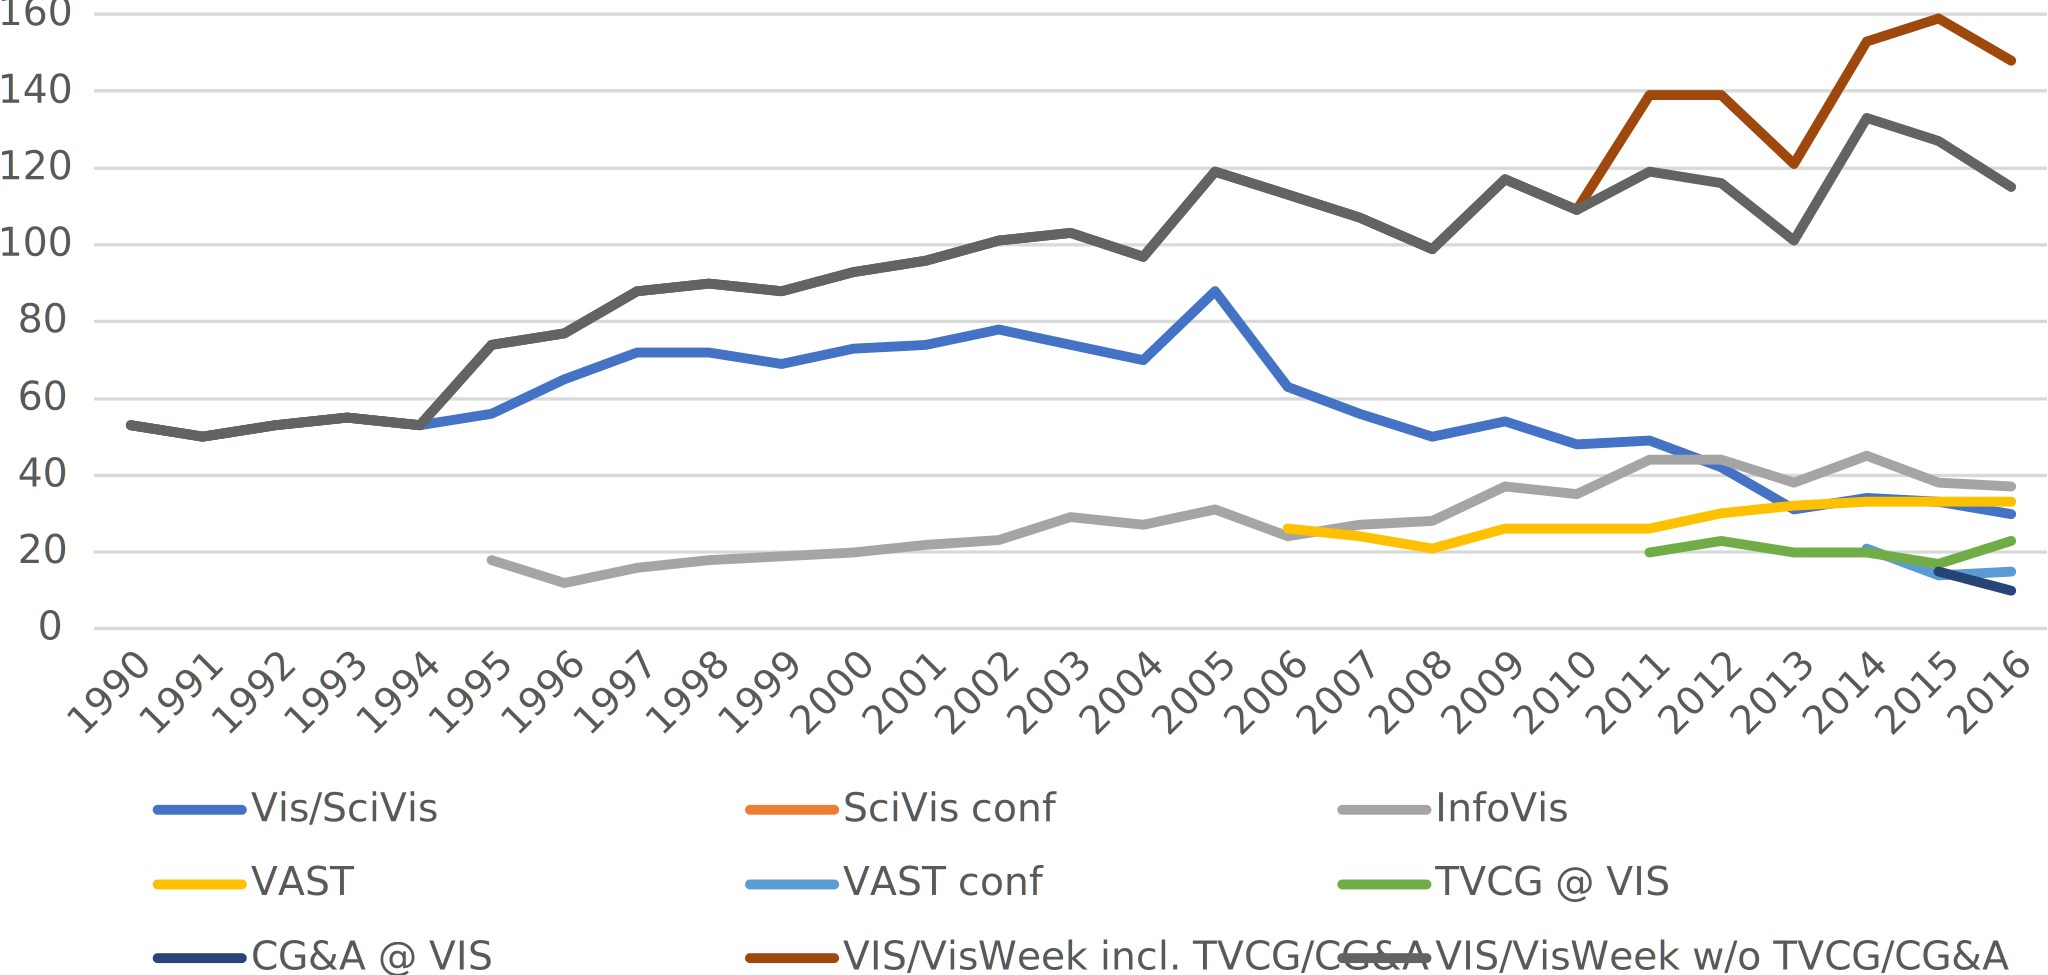
\includegraphics[width=\columnwidth]{paper-count-2016}
%  \caption{A visualization of the 1990--2016 data from \cref{tab:vis_papers}, recreated based on Fig.\ 1 from \cite{Isenberg:2017:VMC} and is in the public domain.}
%  \label{fig:vis_papers}
% \end{figure}

% \subsubsection{Filler Subsubsection to Flush Out the Paper}

% Duis autem~\cite{Lorensen:1987:MCA}\footnote{The algorithm behind
% Marching Cubes \cite{Lorensen:1987:MCA} had already been
% described by Wyvill et al. \cite{Wyvill:1986:DSS} a year
% earlier.} vel eum iriure dolor in hendrerit
% in vulputate velit esse molestie consequat,\footnote{Footnotes
% appear at the bottom of the column.} vel illum dolore eu
% feugiat nulla facilisis at vero eros et accumsan et iusto odio
% dignissim qui blandit praesent luptatum zzril delenit augue duis
% dolore te feugait nulla facilisi. Lorem ipsum dolor sit amet,
% consectetuer adipiscing elit, sed diam nonummy nibh euismod tincidunt
% ut laoreet dolore magna aliquam erat volutpat.


% \paragraph{Filler Paragraph to Flush Out the Paper}

% Ut wisi enim ad minim veniam, quis nostrud exerci tation ullamcorper
% suscipit lobortis nisl ut aliquip ex ea commodo
% consequat~\cite{Nielson:1991:TAD}. Duis autem vel eum iriure dolor in
% hendrerit in vulputate velit esse molestie consequat, vel illum dolore
% eu feugiat nulla facilisis at vero eros et accumsan et iusto odio
% dignissim qui blandit praesent luptatum zzril delenit augue duis
% dolore te feugait nulla facilisi.


% \section{Conclusion}

% \lipsum[1]%

% \section*{Supplemental Materials}
% \label{sec:supplemental_materials}

% Refer to the instructions for this section (\cref{sec:supplement_inst}).
% Below is an example you can follow that includes the actual supplemental material for this template:

% All supplemental materials are available on OSF at \url{https://doi.org/10.17605/OSF.IO/2NBSG}, released under a CC BY 4.0 license.
% In particular, they include (1) Excel files containing the data for and analyses for creating \cref{tab:vis_papers} and \cref{fig:vis_papers}, (2) figure images in multiple formats, and (3) a full version of this paper with all appendices.
% Our other code is intellectual property of a corporation---Starbucks Research---and there is no feasible way to share it publicly.


% \section*{Figure Credits}
% \label{sec:figure_credits}

% Refer to the instructions for this section (\cref{sec:figure_credits_inst}).
% Here are the actual figure credits for this template:

% \Cref{fig:teaser} image credit: Scott Miller / Special to the Vancouver Sun, January 22, 2009, page A6.

% \Cref{fig:vis_papers} is a partial recreation of Fig.\ 1 from \cite{Isenberg:2017:VMC}, which is in the public domain.

% %% if specified like this the section will be committed in review mode
% \acknowledgments{
% The authors wish to thank A, B, and C. This work was supported in part by
% a grant from XYZ.}

%\bibliographystyle{abbrv}
\bibliographystyle{abbrv-doi}
%\bibliographystyle{abbrv-doi-narrow}
%\bibliographystyle{abbrv-doi-hyperref}
%\bibliographystyle{abbrv-doi-hyperref-narrow}

\bibliography{template}
\end{document}
